
\documentclass[11pt,fleqn]{article} 
\usepackage[margin=0.8in, head=0.8in]{geometry} 
\usepackage{amsmath, amssymb, amsthm}
\usepackage{fancyhdr} 
\usepackage{palatino, url, multicol}
\usepackage{graphicx, pgfplots} 
\usepackage[all]{xy}
\usepackage{polynom} 
%\usepackage{pdfsync} %% I don't know why this messes up tabular column widths
\usepackage{enumerate}
\usepackage{framed}
\usepackage{setspace}
\usepackage{array,tikz}

\pgfplotsset{compat=1.6}

\pgfplotsset{soldot/.style={color=black,only marks,mark=*}} \pgfplotsset{holdot/.style={color=black,fill=white,only marks,mark=*}}
\pgfplotsset{my style/.append style={axis x line=middle, axis y line=
middle, xlabel={$x$}, ylabel={$y$} }}

%axis equal 
\pagestyle{fancy} 
\lfoot{}
\rfoot{3-5 Trig Derivatives}

\begin{document}
\renewcommand{\headrulewidth}{0pt}
\newcommand{\blank}[1]{\rule{#1}{0.75pt}}
\newcommand{\bc}{\begin{center}}
\newcommand{\ec}{\end{center}}
\renewcommand{\d}{\displaystyle}

\vspace*{-0.7in}

%%%%%%%%%intro page
\begin{center}
  \large
  \sc{Section 3-5: Derivatives of Trigonometric Functions}\\
\end{center}
Read Section 3.5. Work the embedded problems. \\
\begin{enumerate}
\item Find the derivative of $f(x)=\frac{1}{3}x^3-\frac{x}{3}+\frac{\pi^2}{3}$. (What's wrong with the answer below?)\\

\textbf{answer:} $f(x)=\frac{1}{3}x^3-\frac{x}{3}+\frac{\pi^2}{3}=\frac{1}{3}\left(x^3-x+\pi^2\right)=\frac{1}{3}(3x^2-1)=f'(x)$


\item (Good review for Midterm) The graph of $f(x)$ is sketched below. Graph its derivative $f'(x)$. Then, use your graph of $f'(x)$ to graph the derivative of $f''(x).$

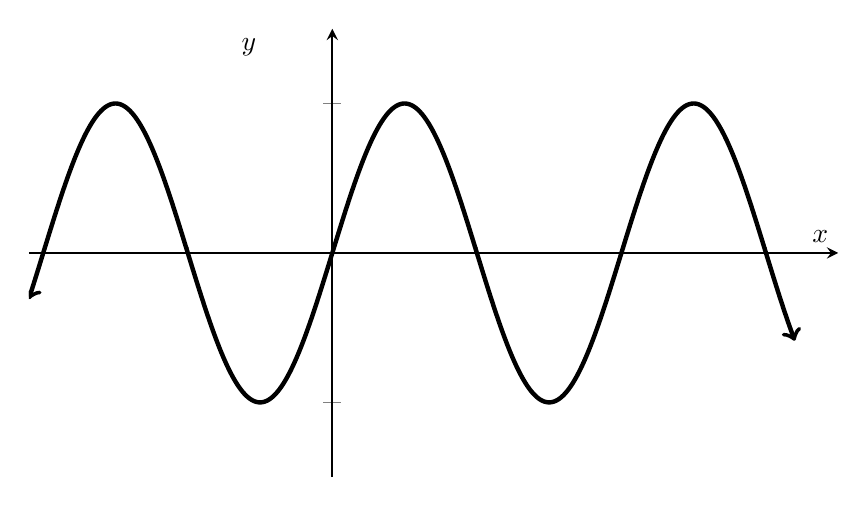
\begin{tikzpicture}
%sine
\begin{axis}[xscale=1.5, thick, my style, xtick={-2,...,3}, ytick={-1,0,1},xmin=-2.1, xmax=3.5, ymin=-1.5, ymax=1.5, yticklabels={,,},xticklabels={,,},
mark size=3.0pt]
\addplot[ultra thick, <->,domain=-2.1:3.2, samples=1000]{sin(180*x)};
\end{axis}
\end{tikzpicture}

\begin{tikzpicture}
%sine
\begin{axis}[xscale=1.5, thick, my style, xtick={-2,...,3}, ytick={-1,0,1},xmin=-2.1, xmax=3.5, ymin=-1.5, ymax=1.5, yticklabels={,,},xticklabels={,,},
mark size=3.0pt]
%\addplot[ultra thick, <->,domain=-2.1:3.2, samples=1000]{sin(180*x)};
\end{axis}
\end{tikzpicture}

\begin{tikzpicture}
%sine
\begin{axis}[xscale=1.5, thick, my style, xtick={-2,...,3}, ytick={-1,0,1},xmin=-2.1, xmax=3.5, ymin=-1.5, ymax=1.5, yticklabels={,,},xticklabels={,,},
mark size=3.0pt]
%\addplot[ultra thick, <->,domain=-2.1:3.2, samples=1000]{sin(180*x)};
\end{axis}
\end{tikzpicture}
\newpage
\item Find the derivative.
	\begin{enumerate}
	\item $y=x^2 + 5 \sin(x)$
	\vfill
	\item $f(\theta) = \theta \cos(\theta)$
	\vfill
	\item $g(x)=\large{\frac{\sin(x)}{x+1}}$
	\vfill
	\item $H(x)=\large{\frac{\sin(x)}{\cos(x)}}$
	\vfill
	\end{enumerate}
\item A mass on a spring vibrates horizontally on a smooth level surface. Its equation of motion is $x(t)=8 \sin(t),$  where $t$ is in seconds and $x$ is in centimeters.\\
	\begin{enumerate}
	\item Find the velocity and acceleration at time $t.$
	\vfill
	\item Find the position, velocity, and acceleration of the mass at time $t=2\pi / 3.$ In what direction is it moving at this time? Is it speeding up or slowing down?
	\vfill
	\end{enumerate}
\end{enumerate}
\end{document}

